\chapter{Progettazione e implementazione} %\label{1cap:spinta_laterale}
% [titolo ridotto se non ci dovesse stare] {titolo completo}
%

\begin{citazione}
    In questo capitolo viene mostrato passo passo un procedimento guida alla realizazzione di un motore scacchistico
\end{citazione}

\newpage
\section{Prefazione} %\label{1sec:scopo}
Lo sviluppo di un motore scacchistico è fortemente influenzato dalle scelte progettuali,
una di queste è il linguaggio di programmazione che si vuole utilizzare,
le prestazioni di un motore possono essere fortemente influenzate dalla natura del linguaggio di
programmazione, in particolare l'utilizzo di un linguaggio interpretato e non compilato può impattare
notevolmente sulla velocità con la quale il nostro motore è in grado di elaborare le milioni di
posizioni con le quali dovrà avere a che fare in una singola partita.
Tutti gli esempi di codice all'interno di questa tesi saranno scritti nel linguaggio C, si consiglia
quindi di avere almeno una minima familiarità con tale linguaggio.Si segnalano comunque diversi
tool  per il linguaggio python per chi volesse approcciarsi a questo mondo utilizzando un
linguaggio più beginner friendly  quali:
\begin{itemize}
    \item \textbf{python-chess}: una libreria di python che contiene funzioni di libreria per la rappresentazione
          di scacchiera e pezzi e per la generazione e validazione delle mosse,utile se ci si vuole concentrare
          esclusivamente sulla parte di ricerca e di valutazione  di un motore scacchistico.
    \item \textbf{Sunfish}: un motore scacchistico per principianti scritto nel linguaggio python che
          in sole 111 linee di codice illustra ,in maniera semplificata, l'implementazione della
          gran parte dei concetti  chiave di un motore scacchistico.

\end{itemize}


\section{Rappresentazione della scacchiera e dei pezzi} %\label{1sec:scopo}
Il primo passo dello sviluppo di un motore scacchistico è decidere come si vuole rappresentare
la scacchiera , si tratta di una scelta fondamentale,non solo perché in seguito ci permetterà
di testare le funzioni che andremo a implementare, ma anche perché è nella scacchiera che ,generalmente,
viene conservato lo stato generale della partita.\footnote{per stato di una partita si intendono informazioni come
    informazioni su chi ha diritto di muovere, i permessi di arrocco,lo stato della regola delle 50 mosse etc}
Inoltre il tipo di codifica può influenzare la rapidità
e la facilità col quale possiamo accedere alle informazioni sullo stato corrente dei pezzi
e come vedremo in seguito è in grado di influenzare funzioni come la generazione delle mosse.
Non è raro per motori scacchistici particolarmente complessi l'utilizzo di più tipi di board in base
al tipo di informazione da conservare e all'utilizzo che se ne vuole fare.
Per la rappresentazione di una scacchiera sono chiaramente possibili moltissime scelte, di seguito
verranno illustrate alcune tra le più popolari ed utilizzate.

\subsection{Rappresentazione Pezzocentrica}
Si definisce rappresentazione pezzocentrica, un qualsiasi tipo di rappresentazione della scacchiera che mantiene liste
array o set dei pezzi attualmente presenti sulla scacchiera con annesse le informazioni sulle caselle da essi occupate.
Le rappresentazioni più comuni sono:
\subsubsection{Piece-Lists}
liste o array di ogni pezzo sulla scacchiera,ogni elemento della lista o dell'array associa un pezzo
alla casella che esso occupa .le caratteristiche di ogni pezzo (colore,tipo etc)
possono essere associate all'indice dell'array in cui si trovano o essere presenti in ulteriori array
o liste esterne. \emph{un'implementazione pratica di una Piece-List verrà mostrata in seguito all'interno
    di questo capitolo}

\subsubsection{Bitboards}
Una Bitboard è una struttura dati specifica per i giochi da tavolo,
si tratta in sostanza  di una struttura dati in grado di immagazzinare lo stato di ogni casella della
scacchiera all'interno di una parola \footnote{Una parola è un gruppo di bit di una determinata dimensione che sono gestiti come unità dal set di istruzioni o dall'hardware di un processore} di 64 bit.
Vediamo un esempio pratico, immaginiamo di avere una scacchiera che si trova nello stato di default di inizio
partita:\\
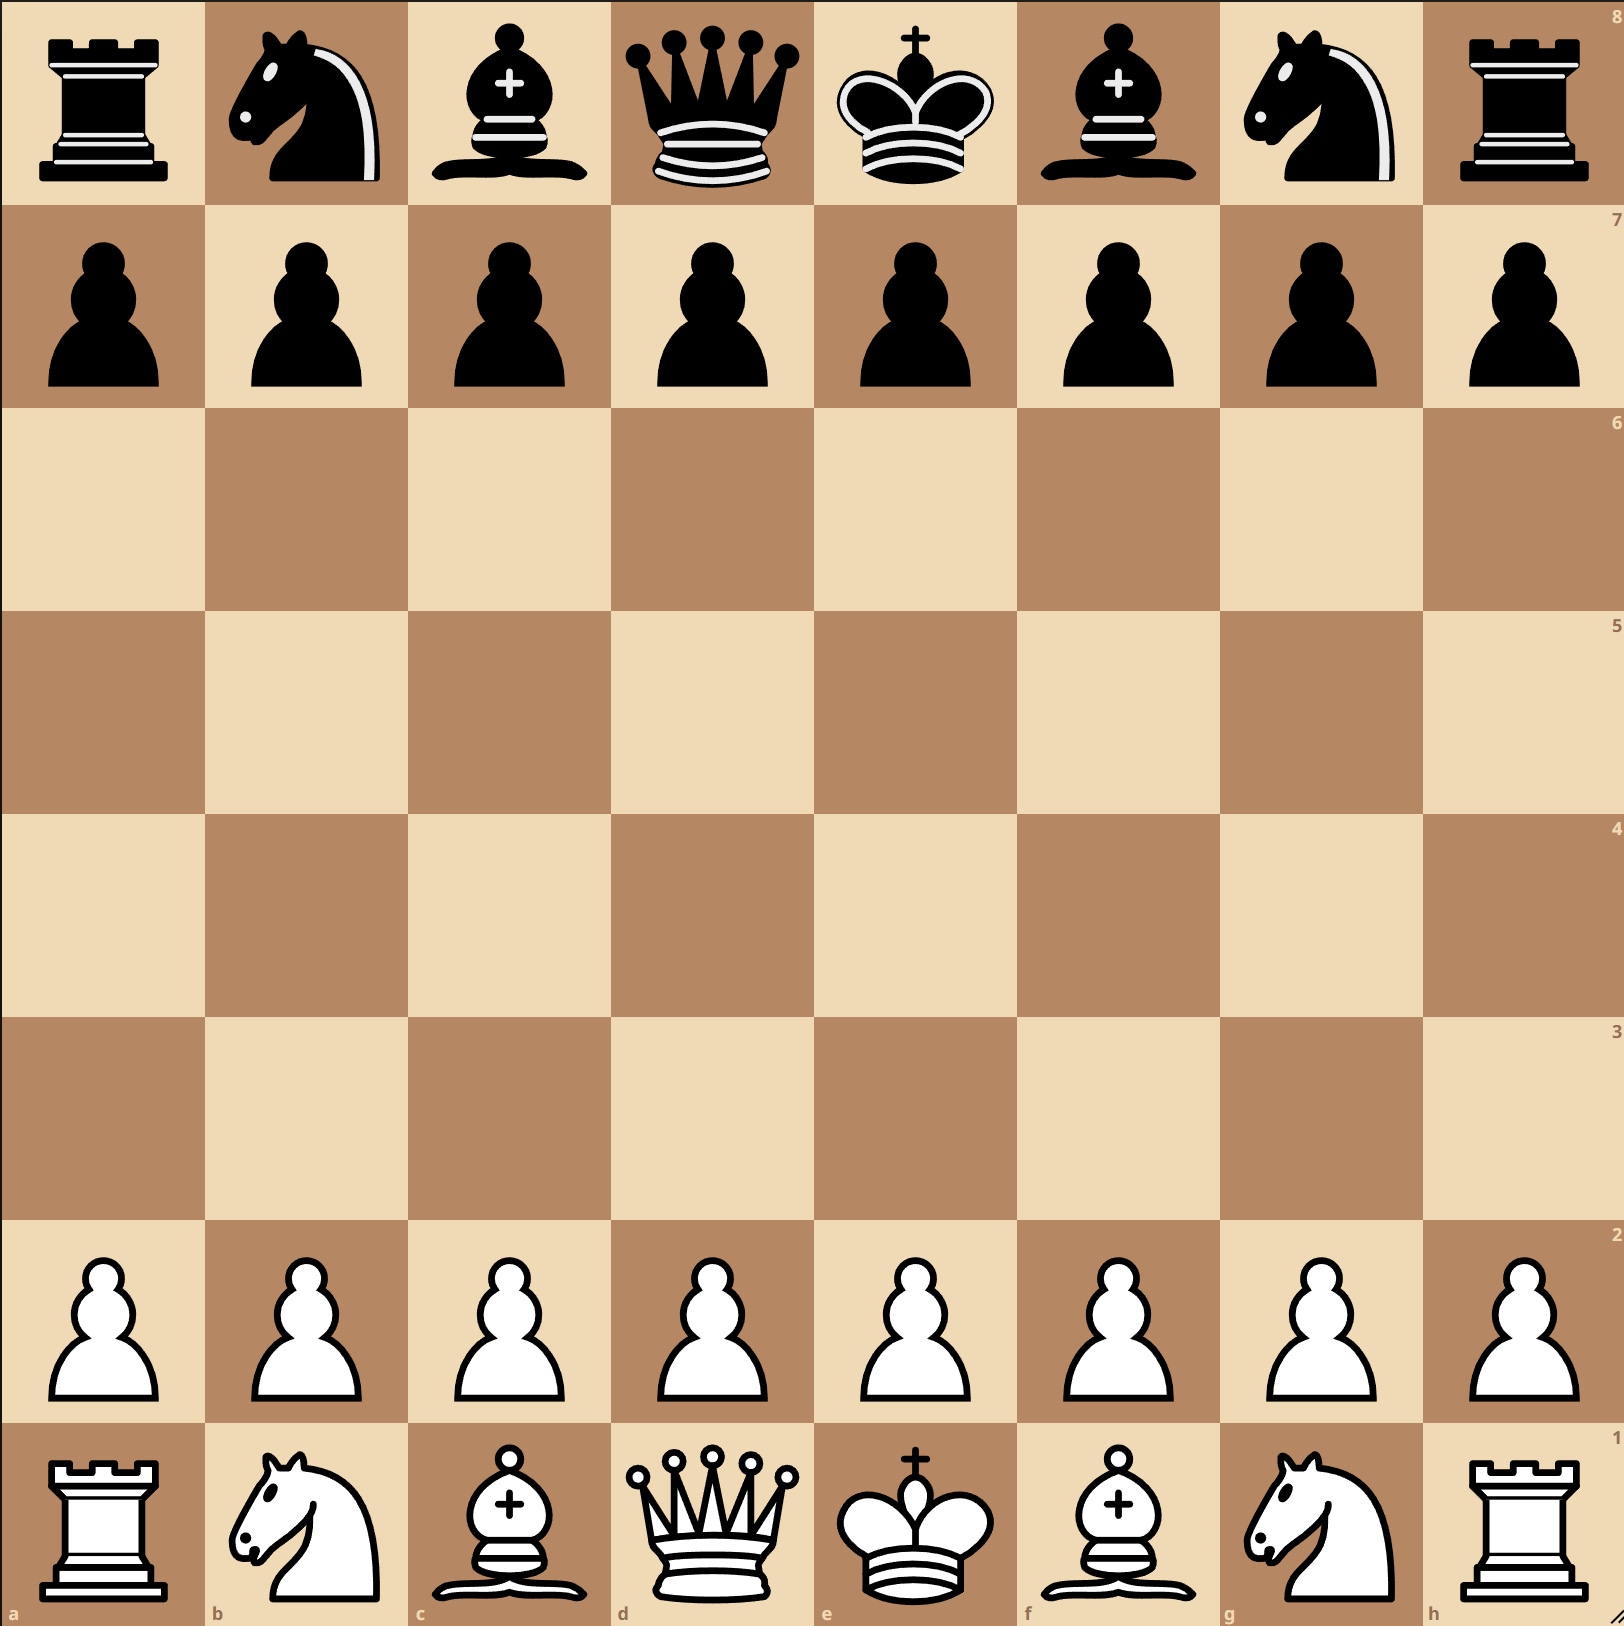
\includegraphics[width=\linewidth] {scacchiera.png}\\
Una bitboard tipica è quella che ci permette di sapere in quali caselle è presente un pedone
nero,per costruirla, operando casella per casella, ci poniamo una domanda "in questa casella
è presente un pedone nero?" se si allora quella casella viene marcata con un 1 , altrimenti viene
marcata con uno 0, il risultato di questa traduzione diventa in questo caso:\\
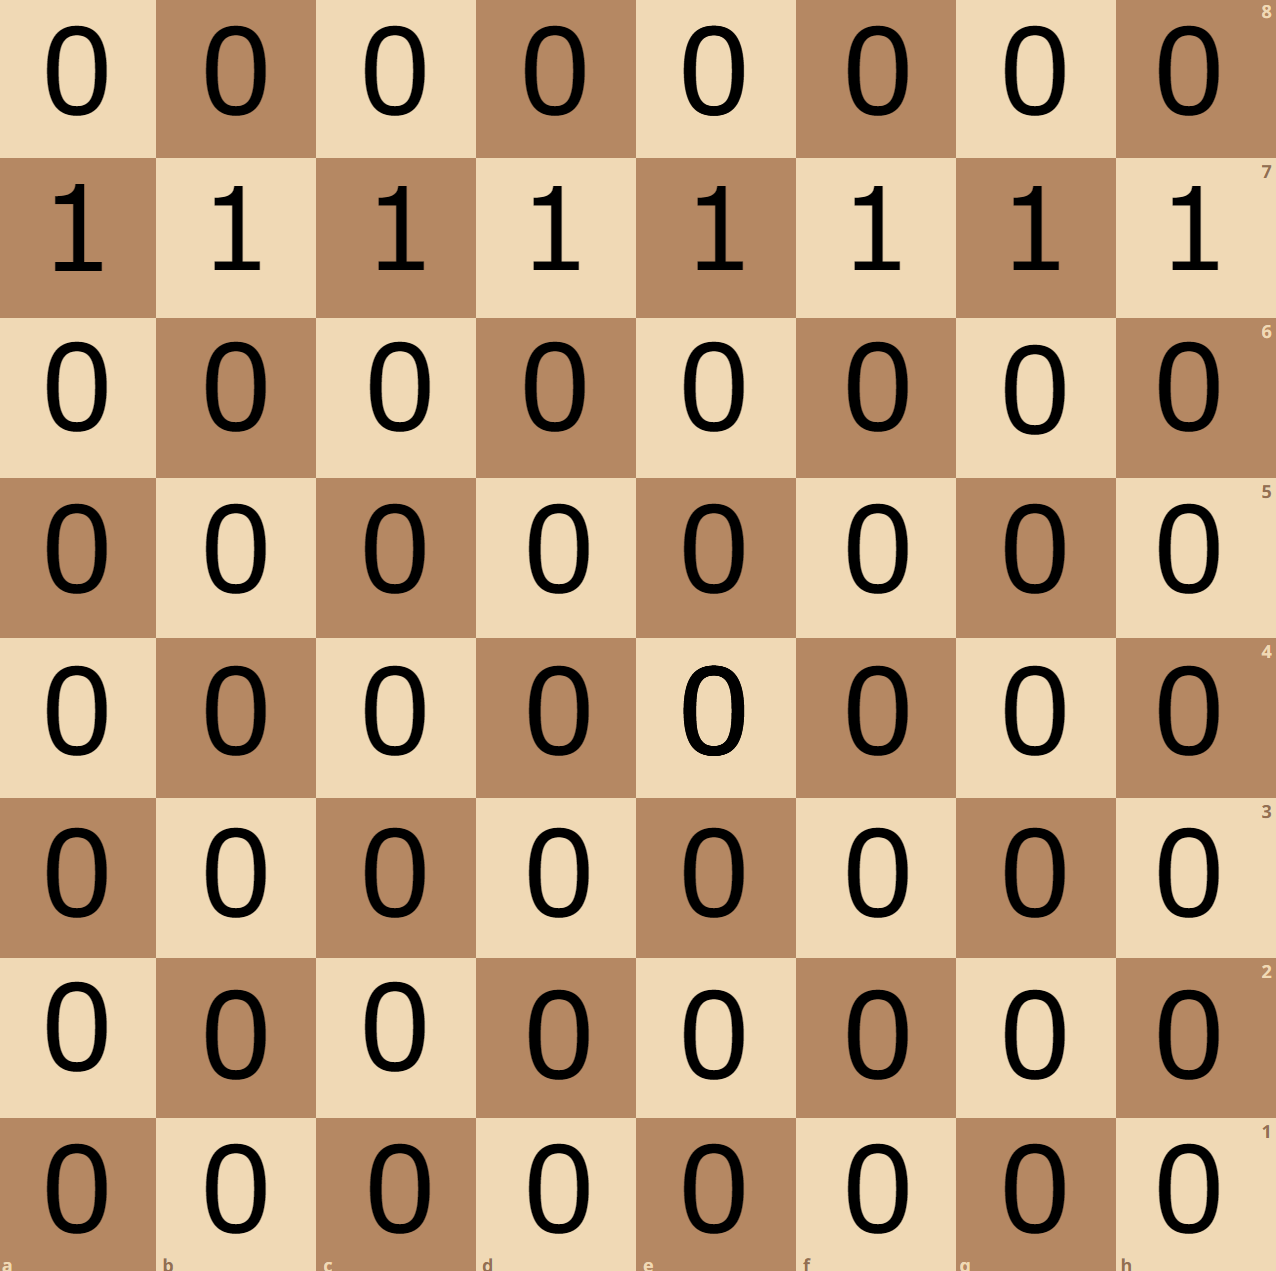
\includegraphics[width=\linewidth] {bitboard.png}\\
La bitboard che codifica questa informazione sarà quindi la parola di 64 bit 00000000 11111111 00000000 00000000 00000000
00000000 00000000 00000000
\subsubsection{Piece-Sets}
rappresentazione con set con un bit per ogni pezzo dentro una parola a 32 bit o 2 parole a 16 bit per ogni lato.
i Piece-sets hanno  delle somiglianze con le bitboards, ma ogni  bit del set non è   direttamente correlato ad una casella,
ma ad un indice  dentro ad una  piece-list. Spesso la bit-position di un  piece-set  implica
, di che tipo e colore il pezzo è. - mentre le  bitboards solitamente mantengono set distinti
per pezzi diversi.
\newpage
\vfill

\begin{figure}
    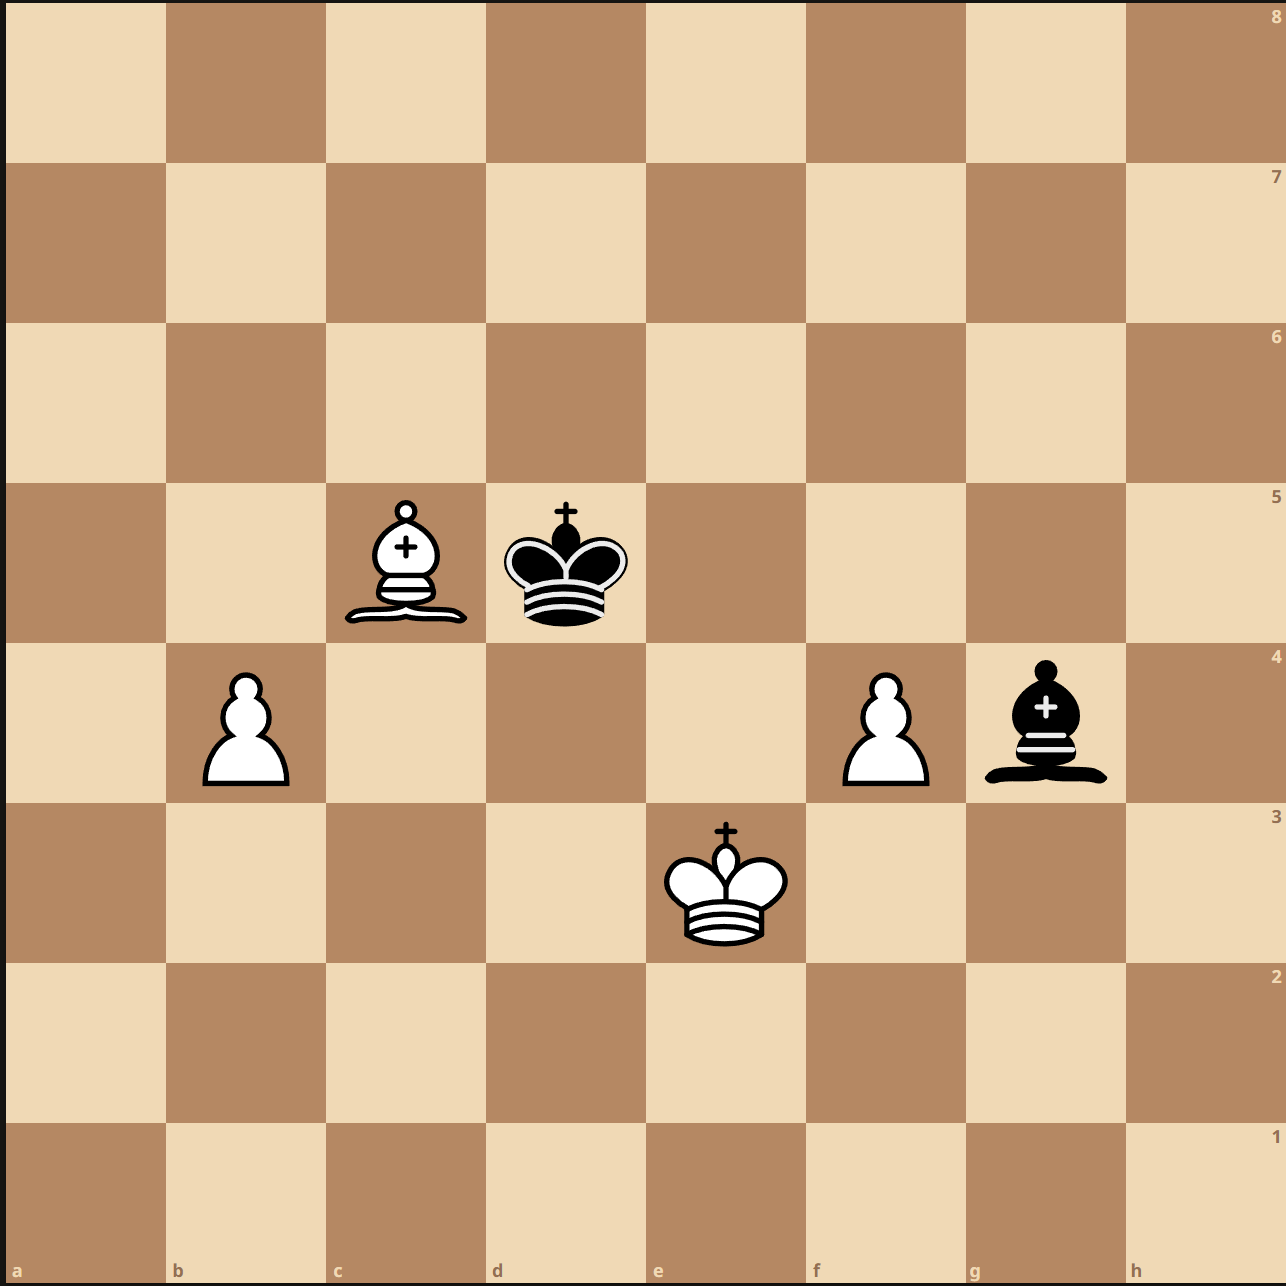
\includegraphics[width=\linewidth]{board.png}
    \caption{Scacchiera nella classica posizione di finale con alfieri di colore opposto }
    \label{board}
\end{figure}

\begin{figure}
    \centering
    
\includegraphics[scale=0.2]{placeholder.png}
    \caption{Rappresentazione set-wise della scacchiera \ref{board} }
\end{figure}

\vfill
\clearpage


\subsection{Rappresentazione Casellocentrica}
La rappresentazione casellocentrica invece mantiene un associazione inversa rispetto a quella pezzocentrica,
per ogni casella conserviamo in memoria se è vuota o occupata da un pezzo in particolare.
La macro-categoria di  rappresentazione più comune è la Mailbox:

\subsubsection{Mailbox}
La rappresentazione Mailbox è una rappresentazione casellocentrica dove la codifica di ogni casella risiede in una struttura dati
che permette l'accesso casuale ,solitamente si utilizza un array con l'indice che codifica dal numero della casella in array monodimensionali
o dalla coppia traversa/colonna\footnote{termini scacchistici per indicare le righe e le colonne della scacchiera} in array bidimensionali.
Il nome deriva dall'associazione di ogni indice al concetto di "indirizzo" di una casella postale.Le implementazioni più famose e
comuni del concetto di Mailbox sono la 8x8 Board, la 10x12 Board e la Vector Attacks.

\subsubsection{8x8 Board}
Una board 8x8 è una rappresentazione pezzocentrica consistente o in un array bidimensionale di bytes o interi, contenenti rappresentazioni codificate
per i pezzi e per la casella vuota, con i due indici ricavati dalla coppia traversa/colonna che identifica la casella sulla scacchiera , 
o più comunemente un array monodimensionale con indici da 0 a 63,uno per ogni casella della scacchiera.
Questo tipo di rappresentazione è usata spesso come rappresentazione ridondante all'interno di programmi che utilizzano bitboards
per individuare se e quali pezzi sono presenti su una casella in maniera efficiente.\\
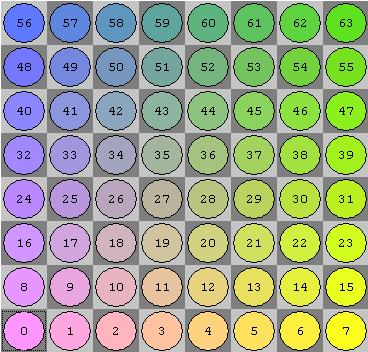
\includegraphics[width=\linewidth]{8x8 board.png}

\subsubsection{10x12 Board}
Una board 10x12  contorna una  board 8x8   con traverse e colonne sentinelle  per individuare  indici off the board while generating moves
using offsets per piece and direction to determine move target squares. Two ranks at the bottom and top are necessary to ensure even knight jumps
from the corners result in valid array indices greater or equal zero and less than 120.

\subsubsection{Vector Attacks}
the application of vectors in the Chebyshev vector space of a chessboard to the problem of chess attacks, including static exchange evaluation (SEE)
, and testing whether moves are pseudo-legal.

\subsubsection{0x88}
a square centric board representation. It uses one nibble for both rank and file each, to index the piece- or empty square codes. While the doubled
array size is negligible, the redundancy of the bit-gaps pays off for several applications. 0x88 is C-syntax and the hexadecimal value of a mask of
bits need to be zero for valid square coordinates (136 decimal, 210 octal, 10001000B).





\section{Move Generation} %\label{1sec:scopo}


\section{Ricerca} %\label{1sec:scopo}

\section{Valutazione} %\label{1sec:scopo}

\section{libro delle aperture,Tablebases} %\label{1sec:scopo}

